% AAAI-27 anonymous submission draft.
% Place the official AAAI-27 author kit files in this directory before final
% submission. Without them, this file uses aaai2027_fallback.sty only so the
% current text can be built and reviewed locally.
\documentclass[letterpaper]{article}
\IfFileExists{aaai2027.sty}{\usepackage{aaai2027}}{\usepackage{aaai2027_fallback}}

\usepackage{amsmath,amssymb,booktabs,multirow}
\usepackage{graphicx}
\usepackage{url}
\usepackage{microtype}
\usepackage[numbers,sort&compress]{natbib}
\usepackage{enumitem}

\setlist[itemize]{leftmargin=*,topsep=2pt,itemsep=1pt}
\setlist[enumerate]{leftmargin=*,topsep=2pt,itemsep=1pt}

\newcommand{\csi}{\mathrm{CSI}}
\newcommand{\TopK}{\mathrm{TopK}}
\newcommand{\Jacc}{\mathrm{J}}
\newcommand{\E}{\mathbb{E}}
\newcommand{\Var}{\mathrm{Var}}

\title{Calibration Split Instability in Mixed-Precision LLM Quantization}
\author{Anonymous Submission}
\affil{Paper ID withheld for double-blind review}

\begin{document}
\twocolumn[
\maketitle
\begin{abstract}
Mixed-precision post-training quantization (PTQ) often turns a small
calibration set into a high-stakes allocation decision: which modules should
receive scarce high-bit precision? We argue that a key failure mode is not only
low final accuracy, but behavior associated with \emph{decision instability}:
equally plausible calibration splits can induce materially different
sensitivity rankings and therefore different allocations under the same bit
budget. Calibration Split Instability (CSI) provides a signal for estimating
calibration-induced instability in PTQ systems, rather than a standalone metric
or a new quantization backend. CSI audits seed-pair agreement using rank
correlation, top-$k$ overlap, positive-set overlap, bootstrap trend tests, and
permutation-null tests before a calibration-derived allocation is promoted from
diagnostic evidence to a stronger method claim. Across Qwen2.5 same-prompt-pool
artifacts, increasing calibration size correlates with higher stability: for Qwen2.5-1.5B,
mean Spearman rises from 0.1410 at $n=2$ to 0.4918 at $n=8$, with positive
bootstrap gain intervals and Holm-adjusted permutation $p \leq 0.00015$. A
stricter second-pool SmolLM2-360M replication shows the same trend from $n=4$
to $n=16$, with mean Spearman improving from 0.3133 to 0.6959 and
Holm-adjusted permutation $p=0.0005999$. We further separate quantization
backends from decision-layer evidence by confronting native PTQ baselines on
full Qwen2.5-1.5B downstream benchmarks: on MMLU (14,042 examples),
FP16/AutoAWQ/GPTQModel reach 0.5864/0.5648/0.5362, and on GSM8K (1,319
examples), 0.0811/0.0788/0.0728. Local GPU fake-quant smokes exercise the
CSI/consensus allocation path without upgrading it to a SOTA claim. The result
is an audit framework that characterizes calibration regime shift, provides
indication of allocation risk, and routes each claim to the evidence required
before stronger downstream claims can be asserted.
\end{abstract}
\keywords{post-training quantization, calibration robustness, mixed precision, large language models, reproducibility}
\vspace{0.7em}
]

\section{Introduction}

Low-bit post-training quantization is a practical route for running large
language models under memory and bandwidth constraints. In mixed-precision PTQ,
however, compression quality depends on a discrete decision made before the
final task score is known: which modules deserve scarce high-bit budget? Uniform
quantization avoids that decision by treating every module equally, but
calibration-driven allocation must infer a module ordering from a small prompt
sample. When the ordering changes under another plausible split, PTQ failure
can be viewed as being associated with decision instability under calibration
shift and the same resource constraint.

This makes calibration instability a reliability concern for any method whose
claim depends on \emph{which} layers, blocks, or channels are protected.
Existing PTQ backends can be strong while still not explicitly modeling
instability boundaries in calibration-driven allocation: they may optimize
reconstruction, rescale activations, learn transforms, or protect salient
channels, but they do not necessarily characterize whether the upstream
calibration-derived allocation would be similar under a nearby calibration draw.
Our novelty anchor is therefore the following: \emph{we treat
calibration-driven PTQ allocation as an auditable process whose claims are
checked against stability, retention, and resource evidence}. A low-bit
allocation is more credible when the ranking is stable across plausible splits,
the retained model behavior passes an evaluation threshold, and the resource
budget is respected.

Many calibration-driven pipelines answer this question by estimating module
sensitivity on a small prompt set, ranking modules, and protecting those that
appear most sensitive. This decomposition is convenient, but it hides a
failure mode. If two small calibration samples drawn from the same prompt pool
produce different sensitivity rankings, a single-split allocation can look
principled while encoding sampling noise. Such instability matters even when
the final quantization backend is strong: GPTQ, AWQ, SmoothQuant, OmniQuant,
QuaRot, and SpinQuant define powerful ways to transform or quantize weights and
activations \citep{frantar2023gptq,lin2024awq,xiao2023smoothquant,shao2024omniquant,ashkboos2024quarot,liu2024spinquant},
but a mixed-precision allocation layer still benefits from evidence that its
calibration-derived ranking is consistent enough to support stronger claims.

This paper studies \emph{calibration split instability} (CSI) as such an
instability signal. CSI is not a new quantization backend and not a direct claim
of state-of-the-art PTQ quality. It is a scoring function used to quantify
calibration-induced instability before calibration-derived decisions are used to
allocate precision. CSI is deliberately positioned
between calibration-data studies and final task-retention benchmarking:
calibration data can affect compression outcomes \citep{calibrationimpact2023},
and benchmark toolkits emphasize standardized evaluation \citep{llmc2024}; CSI
targets the intermediate ranking/allocation instability that can make those
outcomes difficult to interpret.

\begin{figure}[t]
\centering
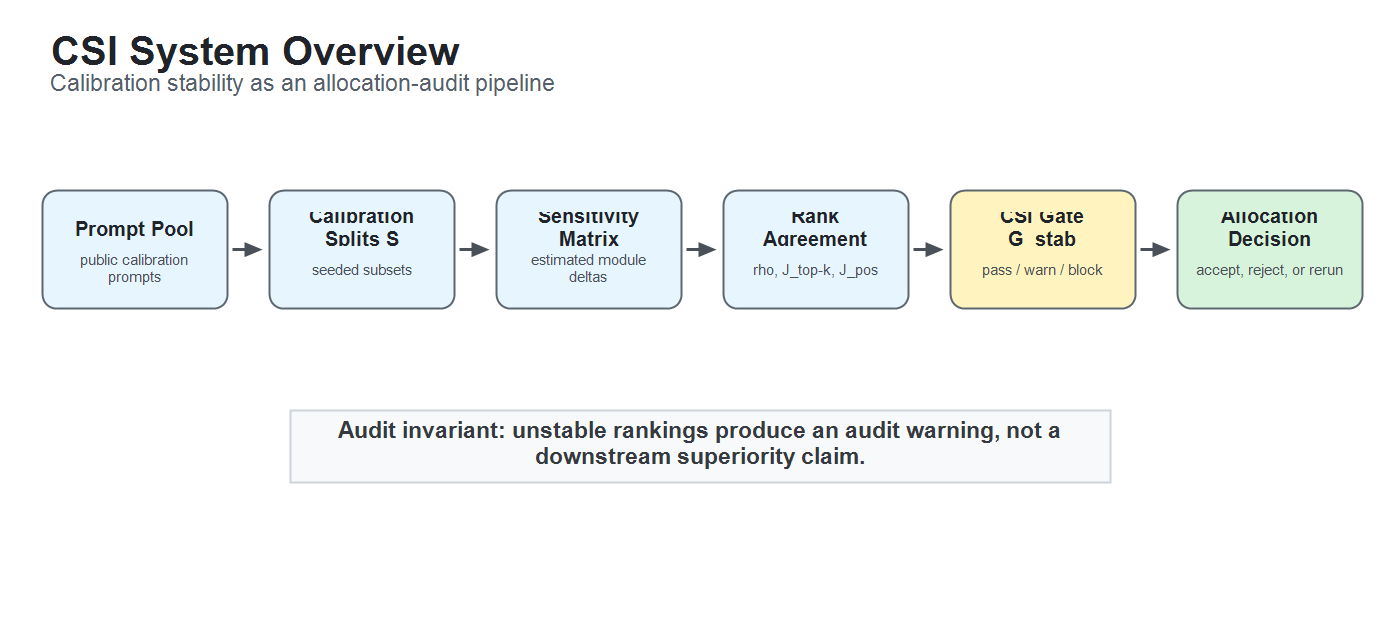
\includegraphics[width=\linewidth]{figures/fig1_pipeline.png}
\caption{CSI audit loop. Calibration splits feed an instability score that
informs an allocation policy before stronger claims are made. Downstream
outcomes do not retroactively prove calibration stability; they update the claim
boundary and future thresholds.}
\label{fig:framework}
\end{figure}

\paragraph{Contributions.}
We make three claims. First, we characterize calibration regime shift as an
instability pattern associated with mixed-precision PTQ allocation: at small
calibration sizes, a single calibration ranking can encode sampling noise while
still appearing methodologically precise. Second, we propose CSI as a scoring
function that provides indication of this instability and supports operational
states such as reject, audit-only, or downstream-validation candidate. Third, we
organize the current evidence into a failure-space audit: native PTQ backends,
CSI allocation smokes, low-bit scaffolds, and failure heatmaps are separated by
what they can and cannot support, reducing the risk that metric evidence is
misreported as downstream quality evidence.

\section{Problem Setup}

Let a transformer have quantizable modules
$\mathcal{M}=\{m_1,\ldots,m_L\}$. A mixed-precision allocation is
$a=(b_1,\ldots,b_L)$, where each bit width $b_i$ belongs to a finite set
$\mathcal{B}$, such as $\{4,8\}$. Let
$C=\{C_1,\ldots,C_S\}$ be calibration splits sampled from a prompt pool. For
split $C_s$, a sensitivity probe estimates the loss increase caused by lowering
the precision of module $m_i$:
\begin{equation}
\hat{\Delta}_{i,s}
= \ell(f_{a^{(i\downarrow)}};C_s)-\ell(f_{a^{ref}};C_s),
\end{equation}
where $a^{ref}$ is a reference allocation and $a^{(i\downarrow)}$ modifies the
probe precision of module $m_i$. A single-split method ranks modules using one
column of $\hat{\Delta}$. CSI asks whether those columns agree.

For each split pair $(s,t)$, we compute a rank agreement score and two set
overlaps:
\begin{align}
\rho_{s,t} &= \mathrm{Spearman}(\hat{\Delta}_{:,s},\hat{\Delta}_{:,t}),\\
\Jacc^k_{s,t} &=
\frac{|\TopK_s(k)\cap\TopK_t(k)|}{|\TopK_s(k)\cup\TopK_t(k)|},\\
\Jacc^{pos}_{s,t} &=
\frac{|P_s\cap P_t|}{|P_s\cup P_t|},
\end{align}
where $P_s=\{i:\hat{\Delta}_{i,s}>0\}$. We report pairwise means and bootstrap
confidence intervals over seed pairs. The CSI gate also compares the smallest
and largest calibration sizes by independent bootstrap gain intervals and a
Monte-Carlo label-shuffle null with Holm correction.

\paragraph{Intended use.}
The statistic above is most relevant for claims that use calibration to choose a
non-uniform allocation. If an allocation ignores calibration, CSI may be less
informative; if a method uses calibration only inside a backend reconstruction
objective, CSI audits only the external allocation or protection decision. This
restriction makes CSI a calibration-instability signal for allocation studies,
not a universal quality metric for every PTQ algorithm.

\paragraph{Composite audit signal.}
Within this decision class, CSI is a composite scoring function rather than a
theoretically exact boundary estimator. A calibration-driven allocation policy
often depends on three observable decisions: the relative module order, the
protected top-$k$ set, and the sign of measured sensitivity. Reporting
$(\rho,\Jacc^k,\Jacc^{pos})$ characterizes these complementary views: rank
agreement, protected-set overlap, and sign consistency. The tuple therefore
indicates allocation-changing perturbations without claiming complete detection
or final task conclusions.

\paragraph{Baseline class framing.}
The comparison classes are not interchangeable. GPTQ, AWQ, SmoothQuant,
OmniQuant, QuaRot, and SpinQuant are backend families; uniform quantization is a
no-allocation baseline; and budget-matched random allocation removes the
calibration term. CSI addresses the remaining class: pipelines that use
calibration to decide \emph{which} modules to protect. It is therefore reported
as an instability signal alongside native PTQ backends, not as their
replacement.

\section{CSI as an Instability Score}

CSI summarizes calibration evidence as an instability score that can inform
operational decisions. We use three non-exclusive reporting states:
\textsc{Reject} for evidence with high measured instability, \textsc{AuditOnly}
for evidence that supports a bounded audit claim but lacks direct downstream
retention, and \textsc{Validate} for candidates that have also passed
fixed-budget downstream evaluation. These states are implementation choices for
claim management, not theoretically exact stability regions.

The stability part of the operator can be used as a hard gate or as a soft
allocation risk. Let
\begin{equation}
\mathcal{G}_{stab}(a;C)=
w_{\rho}\bar{\rho}+w_k\overline{\Jacc^k}+w_p\overline{\Jacc^{pos}}.
\end{equation}
An allocation is stability-admissible only if
$\mathcal{G}_{stab}(a;C)\geq\tau_s$. A smooth risk version is
\begin{equation}
\phi_s(a)=\log\!\left(1+\exp\left(\gamma_s(\tau_s-\mathcal{G}_{stab}(a;C))\right)\right).
\end{equation}
Equivalently, one may read
$p_s(a)=\sigma(\gamma_s(\mathcal{G}_{stab}(a;C)-\tau_s))$ as a soft
probability that the stability gate accepts the allocation. This probabilistic
view is useful operationally: a saturated low $p_s$ indicates calibration
collapse, while high $p_s$ with poor retention indicates that stable rankings
are not enough for quality.
The full constrained calibration objective can be written as
\begin{align}
\min_{a\in\mathcal{B}^L}\quad
\mathcal{J}(a) &=
\mathcal{L}_{task}(a;D)+\lambda_c\mathcal{L}_{cal}(a;C)
\nonumber\\
&\quad + \lambda_s\phi_s(a)+\lambda_u\mathcal{R}_{uncert}(a;C)
\nonumber\\
&\quad + \lambda_b\mathcal{R}_{budget}(a)\\
\text{s.t.}\quad
&\sum_i \mathrm{mem}(m_i,b_i)\leq M,\quad
\mathcal{G}_{ret}(a;D_{val})\geq\tau_r.
\end{align}
This objective separates evidence into the same practical reporting states. If
the stability score is weak, the calibration evidence is treated as
under-supported. If the stability score is stronger but direct retention is
missing, the evidence remains audit-only. If both stability and retention pass
under a fixed budget, the allocation can be discussed as a downstream-validated
candidate. The current paper establishes the first two parts of this pipeline at
scale and reports matched native-PTQ downstream retention rows. It does not yet
claim that a CSI-informed allocation changes those downstream rows end to end.

\paragraph{Propagation argument.}
CSI matters because calibration instability can propagate through the allocation
map. Let $\pi_s$ be the module order induced by split $C_s$ and let
$A(\pi_s,M)$ be the set of modules protected under budget $M$. Low split
agreement can make $A(\pi_s,M)$ and $A(\pi_t,M)$ differ under the same budget,
changing which modules are protected or degraded. Thus calibration size
$\downarrow$ can be associated with rank instability $\uparrow$, allocation
variance $\uparrow$, and downstream-risk exposure $\uparrow$. High CSI does not
establish task success; low CSI suggests rerunning calibration, enlarging the
prompt pool, falling back to a uniform/backend-native policy, or reporting only
an audit failure.

\paragraph{Monotonic stabilization.}
Because $\mathcal{B}^L$ is finite, a search that accepts only improving moves
exhibits monotonic behavior under bounded updates and settles into a local
stable region for the chosen neighborhood. This is a stabilization observation,
not a SOTA-quality theorem.

\section{Experimental Protocol}

\paragraph{Prompt pools and models.}
The Qwen2.5 evidence uses deterministic prompt subsets over a fixed public
WikiText2-style prompt pool \citep{merity2017wikitext,qwen25}. The second-pool
replication uses HuggingFaceTB/SmolLM2-360M-Instruct on a 32-prompt
WikiText2-validation pool \citep{smollm2}. Stress and feasibility rows also
include C4-style text slices \citep{c4}, MMLU \citep{hendrycks2021mmlu}, and
GSM8K \citep{cobbe2021gsm8k}.

\paragraph{Metrics.}
For each calibration size $n$, six deterministic prompt seeds are evaluated.
This yields $15$ seed pairs per $n$. We report mean Spearman, top-20 Jaccard,
and positive-set Jaccard with bootstrap confidence intervals. Trend gates
compare the smallest and largest $n$ values by bootstrap mean-gain intervals
and bootstrap win probabilities. Null gates shuffle the small/large $n$ labels and
apply Holm correction across the three audited metrics.

\paragraph{Native PTQ downstream retention.}
To avoid a purely diagnostic evaluation, we include matched downstream rows for
Qwen2.5-1.5B FP16, AutoAWQ, and GPTQModel variants. MMLU uses all 14,042 test
examples across 57 subjects, and GSM8K uses all 1,319 examples. For each PTQ
candidate, we report accuracy, Wilson intervals, paired bootstrap
candidate-minus-FP16 deltas, and discordant-pair counts from the same task
fixture. These rows confront hard native PTQ baselines, but they are not
CSI-informed allocation rows.

\paragraph{Claim boundary.}
The evidence ledger treats a result as paper-facing only when it has a JSON
artifact, a generated Markdown gate report, a runnable command in the runbook,
and a claim-matrix boundary. Results outside that boundary are discussed only
as future work or local feasibility evidence.

\paragraph{Detect--classify--route protocol.}
Following the claim boundary, experiments are organized around the instability
score rather than around a flat leaderboard. The first layer \emph{detects}
calibration regime shift by measuring how rank and set agreement change with
calibration size. The second layer \emph{classifies} evidence into practical
reporting states such as \textsc{Reject}, \textsc{AuditOnly}, or
\textsc{Validate}-candidate using the CSI score, budget checks, and failure
hooks. The third layer \emph{routes} claims to the evidence they require:
native full-benchmark PTQ rows test downstream retention for backend baselines,
local allocation smokes test the allocation path, and extreme-bit scaffolds mark
regimes that still require direct same-budget downstream evaluation.

\paragraph{Decision-system audit.}
To make the empirical story falsifiable, a claim is promoted only if the
corresponding artifact measures the required regime under the stated boundary.
This prevents a local PPL smoke from being treated as a full MMLU/GSM8K win,
while still making visible where CSI changes allocation behavior and where the
submission-critical rows remain. In this sense, CSI predicts \emph{claim risk}
rather than downstream accuracy directly: low split agreement predicts that an
allocation claim is unsafe to promote, while high agreement only permits the
next validation step.

\paragraph{Policy feedback loop.}
In Figure~\ref{fig:framework}, a calibration pool produces a CSI score, the
score suggests a reporting state, the allocation policy is executed only for
better supported states, and downstream outcomes update thresholds, claim maps,
or rerun decisions.

\paragraph{Mechanism chain.}
The intended explanatory chain is not ``more components give better numbers.''
It is \emph{calibration sampling} $\rightarrow$ \emph{ranking stability}
$\rightarrow$ \emph{reporting-state classification} $\rightarrow$
\emph{retention under a fixed budget}. Each arrow has a falsification hook:
seed-pair CSI tests the first arrow, the instability score informs the second,
fake-quant PPL stress tests whether an allocation path is plausible, and full
MMLU/GSM8K rows test final retention for native PTQ baselines. This
organization prevents a strong final score from hiding unstable calibration
evidence, and prevents a stable ranking from being misreported as downstream
quality evidence before retention is measured.

\section{Results}

\subsection{Claim Boundary and Evidence Promotion}

Figure~\ref{fig:boundary} states the claim-promotion map used throughout the
paper. The map interprets CSI evidence in practical reporting states: unstable
calibration rankings suggest \textsc{Reject}; more stable rankings without
direct task retention suggest \textsc{AuditOnly}; and fixed-budget downstream
retention can move a candidate into a \textsc{Validate} report. Thus diagnostic
evidence can characterize calibration stability, but it cannot by itself
establish that a downstream task score will improve. This framing is
deliberately stricter than a standard result table because it exposes the point
where an attractive allocation result remains under-supported.

\begin{figure*}[t]
\centering
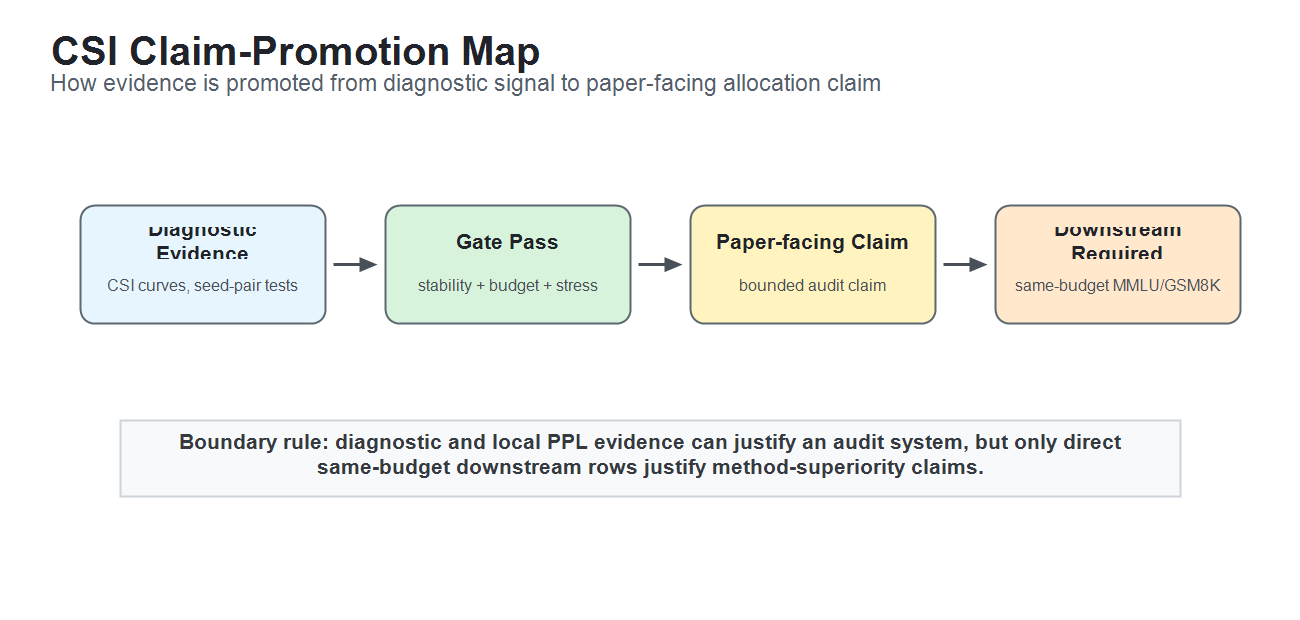
\includegraphics[width=\linewidth]{figures/fig6_boundary.png}
\caption{CSI claim-promotion map for allocation evidence. The framework uses
\textsc{Reject}, \textsc{AuditOnly}, and \textsc{Validate} as practical
reporting states rather than exact theoretical regions. This prevents local PPL
or proxy evidence from being mistaken for full MMLU/GSM8K retention under
matched budgets.}
\label{fig:boundary}
\end{figure*}

\subsection{Calibration Size Correlates with CSI Stability}

Table~\ref{tab:qwen15} shows the Qwen2.5-1.5B same-prompt-pool curve. All three
metrics increase monotonically from $n=2$ to $n=8$. Mean Spearman changes by
0.3508, top-20 Jaccard by 0.1797, and positive-set Jaccard by 0.1747. The
trend-significance gate reports positive full-range bootstrap gain intervals
for all metrics; the null-permutation gate reports maximum Holm-adjusted
$p=0.00015$.

\begin{table}[t]
\centering
\small
\caption{Qwen2.5-1.5B CSI stability over calibration size. Each row uses six
calibration seeds and 15 seed pairs.}
\label{tab:qwen15}
\begin{tabular}{rrrr}
\toprule
$n$ & Spearman & Top-20 Jaccard & Positive Jaccard \\
\midrule
2 & 0.1410 & 0.2604 & 0.4244 \\
4 & 0.2869 & 0.3313 & 0.5189 \\
8 & 0.4918 & 0.4401 & 0.5992 \\
\bottomrule
\end{tabular}
\end{table}

\begin{figure}[t]
\centering
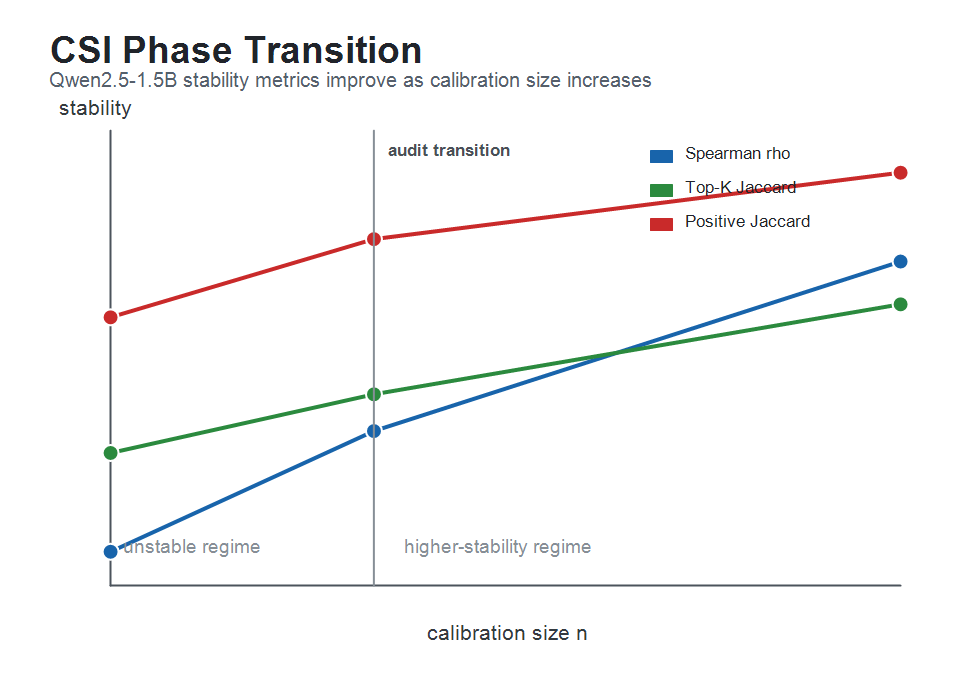
\includegraphics[width=\linewidth]{figures/fig2_phase_transition.png}
\caption{Phase-transition behavior of CSI stability metrics as calibration size
increases on Qwen2.5-1.5B. All three metrics rise from $n=2$ to $n=8$; the
$n=4$ region marks the audit transition where rankings begin moving out of the
low-agreement regime.}
\label{fig:phase-transition}
\end{figure}

Table~\ref{tab:crossscale} compares Qwen2.5-0.5B and Qwen2.5-1.5B at matched
$n$. The 1.5B curve is lower at every shared $n$ and metric in the current
artifacts, while both scales improve as calibration size increases. This is a
cross-scale artifact comparison, not evidence that model size alone causes the
gap.

\begin{figure}[t]
\centering
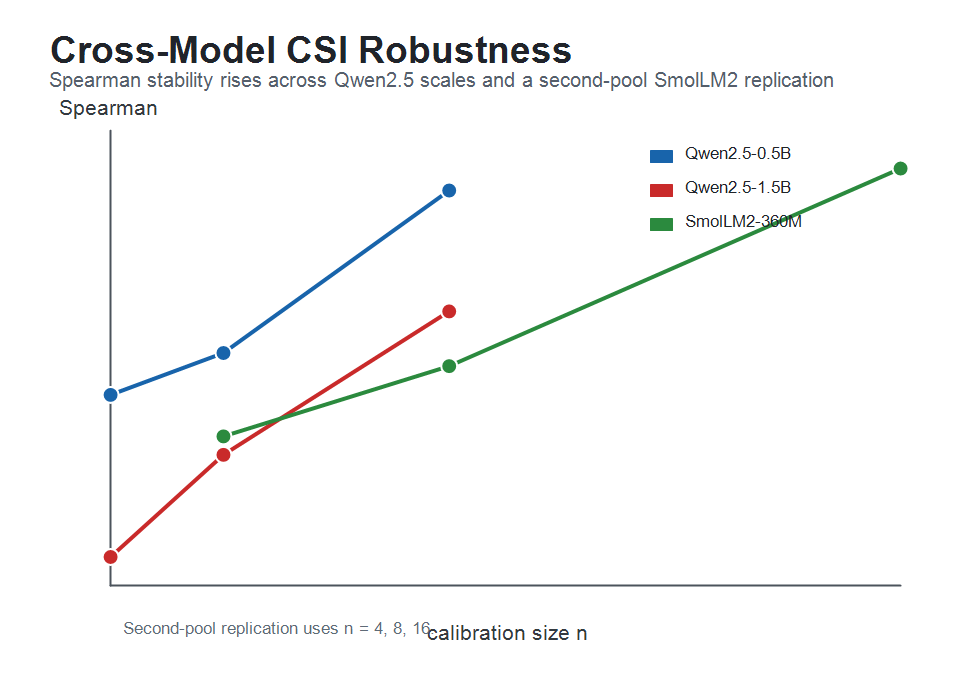
\includegraphics[width=\linewidth]{figures/fig3_cross_model.png}
\caption{Cross-model CSI robustness across Qwen2.5 scales and a second-pool
SmolLM2 replication. The curves are not claimed to be universal, but they show
that increasing calibration size correlates with higher Spearman stability across the current
model and prompt-pool evidence lines.}
\label{fig:cross-model}
\end{figure}

\begin{table}[t]
\centering
\small
\caption{Same-$n$ Qwen2.5 cross-scale CSI comparison. Entries are mean seed-pair
scores.}
\label{tab:crossscale}
\begin{tabular}{rlrrr}
\toprule
$n$ & Metric & 0.5B & 1.5B & Diff. \\
\midrule
2 & Spearman & 0.3725 & 0.1410 & -0.2315 \\
2 & Top-20 & 0.3797 & 0.2604 & -0.1193 \\
2 & Positive & 0.5485 & 0.4244 & -0.1240 \\
4 & Spearman & 0.4324 & 0.2869 & -0.1455 \\
4 & Top-20 & 0.4672 & 0.3313 & -0.1359 \\
4 & Positive & 0.5734 & 0.5189 & -0.0545 \\
8 & Spearman & 0.6645 & 0.4918 & -0.1727 \\
8 & Top-20 & 0.6449 & 0.4401 & -0.2048 \\
8 & Positive & 0.7282 & 0.5992 & -0.1291 \\
\bottomrule
\end{tabular}
\end{table}

\subsection{Second-Pool Replication}

Table~\ref{tab:smollm2} reports the stricter second-pool SmolLM2-360M run. It
uses $n=4,8,16$, six independent seeds per $n$, and all 225 Linear modules per
seed. Mean Spearman rises from 0.3133 to 0.6959. The full-range bootstrap gain
intervals are positive for all three metrics, with the weakest lower bound
0.1395. The permutation-null gate reports maximum Holm-adjusted
$p=0.0005999$.

\begin{table}[t]
\centering
\small
\caption{SmolLM2-360M second-pool CSI stability.}
\label{tab:smollm2}
\begin{tabular}{rrrr}
\toprule
$n$ & Spearman & Top-20 Jaccard & Positive Jaccard \\
\midrule
4 & 0.3133 & 0.3779 & 0.5390 \\
8 & 0.4136 & 0.4363 & 0.5991 \\
16 & 0.6959 & 0.5761 & 0.7512 \\
\bottomrule
\end{tabular}
\end{table}

\subsection{Full Downstream Retention under Native PTQ}

Table~\ref{tab:full-retention} addresses the most direct downstream-evaluation
risk. On Qwen2.5-1.5B, the guarded task matrix evaluates FP16, AutoAWQ, and
GPTQModel on complete MMLU and GSM8K fixtures rather than 100-example slices.
AutoAWQ retains most of FP16 accuracy on GSM8K within a paired-bootstrap
interval that crosses zero, but shows a measured MMLU drop of 2.16 points. The
GPTQModel row drops more on MMLU and slightly on GSM8K. These rows do not show
that CSI allocation raises final quality, but they provide a broader
native-baseline confrontation than a calibration-only or subset-only study.

\begin{table*}[t]
\centering
\small
\caption{Full downstream retention for Qwen2.5-1.5B under matched native PTQ
task fixtures. Deltas are candidate-minus-FP16 paired bootstrap intervals.}
\label{tab:full-retention}
\begin{tabular}{llrrrrr}
\toprule
Task & Variant & $N$ & Acc. & Wilson CI & $\Delta$ vs FP16 & $\Delta$ CI \\
\midrule
MMLU & FP16 & 14042 & 0.5864 & [0.5782, 0.5945] & -- & -- \\
MMLU & AutoAWQ & 14042 & 0.5648 & [0.5566, 0.5730] & -0.0216 & [-0.0273, -0.0155] \\
MMLU & GPTQModel & 14042 & 0.5362 & [0.5279, 0.5444] & -0.0502 & [-0.0570, -0.0432] \\
GSM8K & FP16 & 1319 & 0.0811 & [0.0676, 0.0971] & -- & -- \\
GSM8K & AutoAWQ & 1319 & 0.0788 & [0.0655, 0.0946] & -0.0023 & [-0.0190, 0.0144] \\
GSM8K & GPTQModel & 1319 & 0.0728 & [0.0600, 0.0881] & -0.0083 & [-0.0243, 0.0076] \\
\bottomrule
\end{tabular}
\end{table*}

\subsection{Local GPU CSI-Allocation Smoke}

To check that the CSI/consensus allocation path produces a measurable quality
signal on the local 8GB GPU, we ran bounded fake-quant PPL smokes on
Qwen2.5-0.5B and Qwen2.5-1.5B. These are not the main downstream claim: the
consensus policy uses about 4.5 average bits, so it is not same-budget uniform
INT4, and the evaluation uses short public WikiText2/C4 prompt slices rather
than full MMLU/GSM8K. Nevertheless, it exercises the actual allocation path.
Across four 0.5B local GPU PPL slices, consensus 4-to-8 allocation gives lower
PPL than uniform INT4 in all four cases, with allocation/uniform-INT4 PPL ratios
between 0.7900 and 0.8538. A split-config 1.5B WikiText2 single-slice run shows
the same direction: FP16 10.82, uniform INT4 15.63, and CSI/consensus allocation
13.51 PPL.

\begin{table}[t]
\centering
\small
\caption{Local GPU fake-quant PPL smoke. Lower is better. The consensus
allocation uses about 4.5 average bits, so these rows are directional
feasibility evidence rather than same-budget downstream claims.}
\label{tab:local-smoke}
\begin{tabular}{llrrrr}
\toprule
Model & Slice & FP16 & INT4 & INT3 & CSI alloc. \\
\midrule
0.5B & WikiText2-8 & 24.73 & 41.50 & 915.60 & 32.78 \\
0.5B & C4-8 & 30.64 & 47.26 & 1138.74 & 40.35 \\
0.5B & WikiText2-16 & 25.01 & 42.23 & 804.83 & 32.34 \\
0.5B & C4-16 & 28.85 & 44.86 & 962.40 & 38.21 \\
1.5B & WikiText2-1 & 10.82 & 15.63 & -- & 13.51 \\
\bottomrule
\end{tabular}
\end{table}

\begin{figure}[t]
\centering
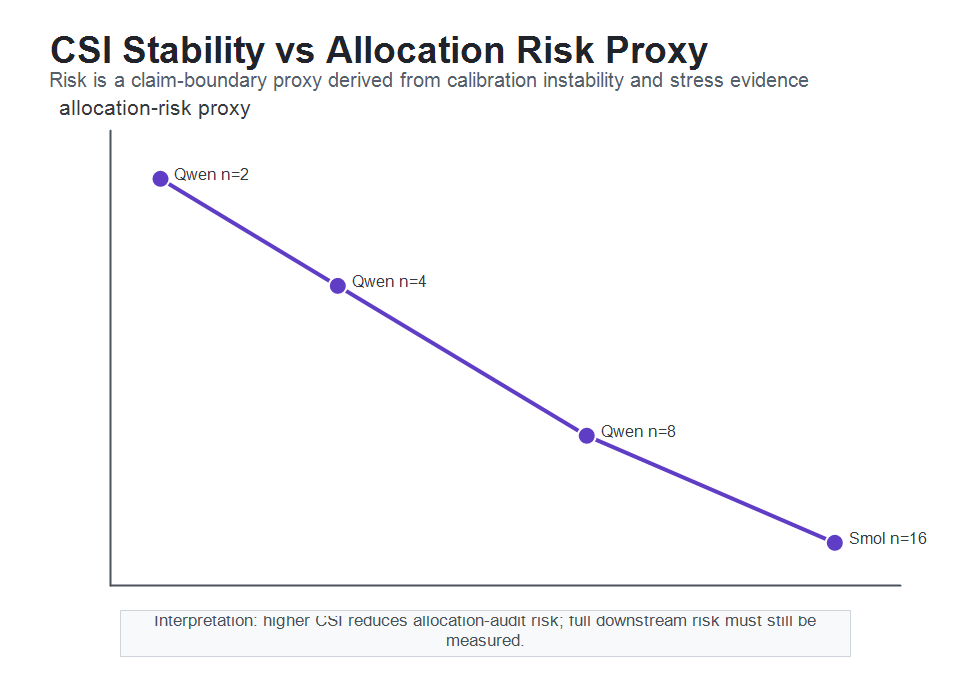
\includegraphics[width=\linewidth]{figures/fig4_risk.png}
\caption{Instability propagation schematic and allocation-risk proxy.
Calibration split noise can propagate into rank instability, allocation
variance, and retention risk. CSI provides a pre-allocation signal: low split
agreement suggests caution, while high agreement indicates that downstream
validation remains the next required step.}
\label{fig:risk}
\end{figure}

\subsection{Consensus Allocation Stress Evidence}

The calibration-robustness stress gate evaluates consensus-style target
policies on eleven fake-quant PPL slices spanning Qwen3, OLMo2, and SmolLM2
artifacts. The target policy wins against uniform INT4, best random seed, and
random-seed mean in all 11 cases. Mean margins are 4.2942 PPL versus uniform,
1.1622 versus best random, and 2.7444 versus random mean, each with one-sided
sign-test $p=0.000488$. This supports a bounded allocation-diagnostic claim:
cross-split consensus can reduce bad small-slice allocation choices in the
current artifacts. It is not a production PTQ or downstream task-retention
claim.

Table~\ref{tab:ablation} maps objective components to the evidence that would
fail or weaken if the component were removed. This is a mechanistic ablation
map rather than a new accuracy table: each row lists the role of a term in the
constrained formulation and the committed gate that exercises that role.

\begin{table}[t]
\centering
\small
\caption{Mechanistic ablation map for the constrained formulation.}
\label{tab:ablation}
\begin{tabular*}{\linewidth}{@{\extracolsep{\fill}}lll}
\toprule
Removed part & Failure mode & Evidence hook \\
\midrule
CSI gate & rank noise & $n=2$ $\rho=0.1410$ \\
Consensus & bad split & $+2.1855$ PPL vs worst \\
Budget term & resource drift & 6 budget-pass cases \\
Interaction & additive miss & 5 swap counterexamples \\
Claim gate & overstated SOTA & RTX3090 as feasibility \\
\bottomrule
\end{tabular*}
\end{table}

Figure~\ref{fig:failure-separation} turns the same logic into a baseline-facing
failure separation map. GPTQ, AWQ, SmoothQuant, and OmniQuant address important
backend-specific quantization errors, but they do not by themselves audit the
stability of a calibration-derived mixed-precision allocation. CSI is therefore
positioned as an orthogonal gate: it lowers split-drift, ranking-collapse, and
constraint-conflict risks, while explicitly leaving the downstream retention
gap open until same-budget task rows are measured.

\begin{figure*}[t]
\centering
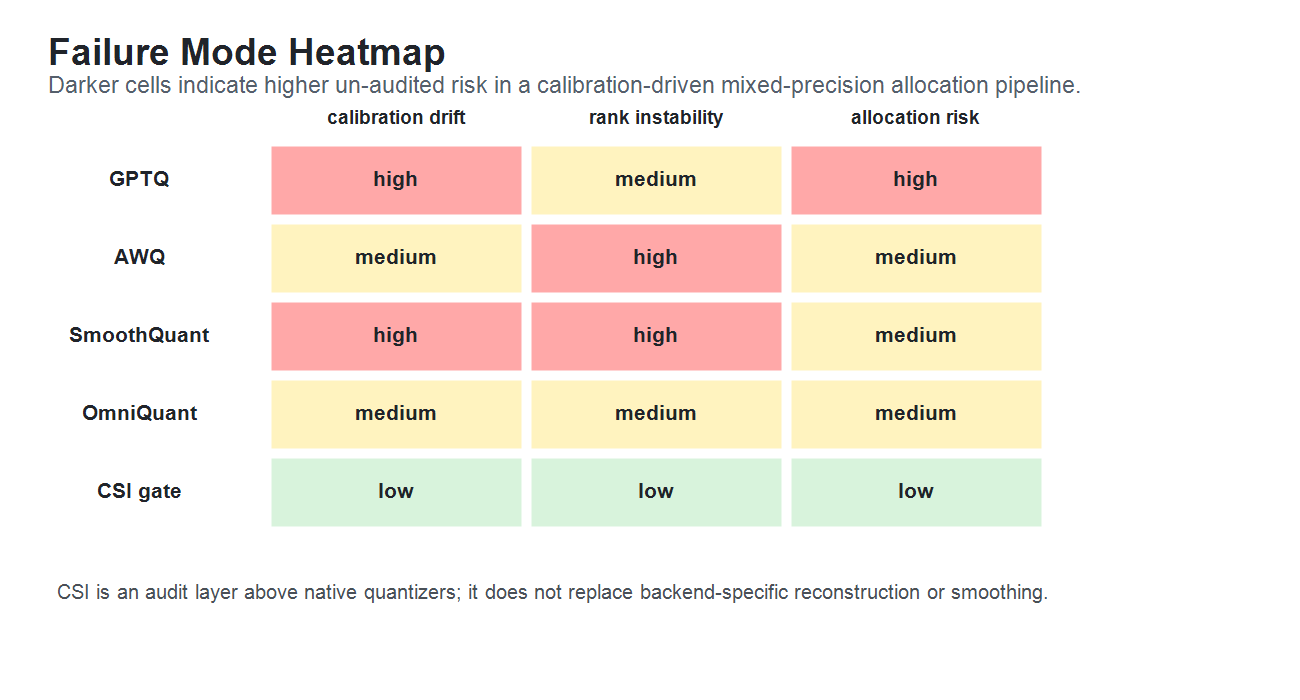
\includegraphics[width=\linewidth]{figures/fig5_failure.png}
\caption{Failure mode heatmap across PTQ method families. Darker cells indicate
higher un-audited risk in a calibration-driven allocation pipeline, not that a
backend is weak in its native setting. CSI is complementary to GPTQ, AWQ,
SmoothQuant, and OmniQuant: it audits the calibration/allocation decision above
the native quantizer.}
\label{fig:failure-separation}
\end{figure*}

\subsection{Extreme-Bit and Failure-Mode Stress}

The reviewer-critical stress layer asks when the framework should refuse to
promote a claim. We separate three failure types. First, \emph{calibration
collapse}: at Qwen2.5-1.5B $n=2$, mean Spearman is only 0.1410, so a
single-split allocation is under-supported. Second, \emph{constraint conflict}:
in the rate-distortion scaffold, uniform INT2 and INT3 produce 16.0$\times$
and 4.0$\times$ the distortion of uniform INT4, while a 2.6-bit
rate-distortion allocation still has 4.904$\times$ uniform-INT4 distortion.
Third, \emph{gate misfire}: in a later random-seed audit, one best random seed
beats the target on a WikiText2 slice by 1.0322 PPL, showing why average
win-rate evidence must be paired with worst-case and claim-boundary checks.
These are not presented as final 2-bit/3-bit task results; they are the current
stress evidence that indicates what should be rerun on larger hardware before a
stronger AAAI claim.

\subsection{Guarded RTX3090 Feasibility Rows}

Table~\ref{tab:rtx3090} summarizes local RTX3090 comparisons for
Qwen2.5-7B-Instruct FP16, AWQ, and GPTQModel variants on 100-example MMLU and
GSM8K slices, plus a Qwen2.5-14B-AWQ 10-example smoke. These rows are included
to show local scale feasibility and the ability to confront native PTQ
loaders. They do not establish leaderboard quality, SOTA PTQ, or production
runtime acceleration.

\begin{table}[t]
\centering
\small
\caption{Local RTX3090 guarded task rows.}
\label{tab:rtx3090}
\begin{tabular}{llrrr}
\toprule
Variant & Task & Limit & Acc. & Tok/s \\
\midrule
7B FP16 & MMLU & 100 & 0.71 & 8.376 \\
7B AWQ & MMLU & 100 & 0.70 & 6.765 \\
7B GPTQ & MMLU & 100 & 0.74 & 7.231 \\
7B FP16 & GSM8K & 100 & 0.24 & 15.263 \\
7B AWQ & GSM8K & 100 & 0.24 & 11.416 \\
7B GPTQ & GSM8K & 100 & 0.16 & 10.828 \\
14B AWQ & MMLU & 10 & 0.50 & 3.851 \\
\bottomrule
\end{tabular}
\end{table}

\section{Related Work}

\paragraph{PTQ algorithms.}
GPTQ uses approximate second-order information for one-shot quantization
\citep{frantar2023gptq}. AWQ protects salient channels using activation-aware
statistics \citep{lin2024awq}. SmoothQuant migrates activation outlier
difficulty into weights for W8A8 inference \citep{xiao2023smoothquant}.
OmniQuant learns clipping and equivalent transforms under calibration samples
\citep{shao2024omniquant}. These are backend families: they answer how to
quantize once a representation or protection policy is chosen. CSI answers a
different question before that policy is executed: whether a
calibration-derived allocation or protection decision shows signs of
instability. Our full Qwen2.5-1.5B rows therefore confront AutoAWQ and GPTQModel
as native PTQ baselines, while CSI is framed as a pre-allocation stability
signal that can be used with such backends rather than as a drop-in replacement
for them.

\begin{table}[t]
\centering
\small
\caption{Failure contrast: what each baseline family primarily leaves
un-audited in a calibration-driven mixed-precision allocation pipeline.}
\label{tab:failure-contrast}
\begin{tabular}{lll}
\toprule
Family & Strength & Unchecked failure \\
\midrule
GPTQ & reconstruction backend & split drift \\
AWQ & salient-channel backend & ranking collapse \\
SmoothQuant & outlier-scaling backend & allocation drift \\
OmniQuant & learned-transform backend & gate conflict \\
CSI & stability signal & retention gap \\
\bottomrule
\end{tabular}
\end{table}

\paragraph{Rotation and outlier handling.}
QuaRot and SpinQuant alter the quantization surface through fixed or learned
rotations \citep{ashkboos2024quarot,liu2024spinquant}. CSI is complementary:
it asks whether calibration-dependent sensitivity or protection decisions are
stable across plausible prompt samples.

\paragraph{Calibration and benchmarking.}
Calibration data has been shown to affect post-training compression outcomes
\citep{calibrationimpact2023}. Benchmarking work such as LLMC argues for
standardized quantization settings \citep{llmc2024}. CSI contributes a narrower
pre-allocation audit signal: before arguing about final task scores, characterize
whether the module ranking used for allocation appears stable.

\section{Limitations and Falsification}

The strongest current evidence is a reproducible CSI measurement and gating
pipeline plus matched native-PTQ downstream retention on full Qwen2.5-1.5B
MMLU/GSM8K fixtures. Local GPU fake-quant smokes now provide directional
allocation-path evidence on Qwen2.5-0.5B and a Qwen2.5-1.5B single-slice run.
We therefore make a system-level audit claim rather than a broad PTQ SOTA
claim: CSI provides indication of whether calibration-derived allocation
evidence appears stable, and it marks the evidence still needed before making
stronger downstream claims.

Before submission, the most important missing row is a direct CSI-informed
downstream retention stress test in the 2--3 bit regime. The current artifacts
contain full 1.5B MMLU/GSM8K native-PTQ retention and local 7B/14B feasibility,
plus uniform INT3 and synthetic INT2/INT3 distortion scaffolds, but they do not
yet contain a full task-retention curve over 2, 3, 4, and 8 bits for FP16,
uniform, native PTQ, and CSI-informed allocations. That experiment should be
run before upgrading the paper from a robustness-plus-retention claim to a
method-quality claim.

Several results could weaken the story. A second public prompt pool could fail
to reproduce the stability trend. Another model family could show stable
rankings even at very small $n$. Downstream task retention could be insensitive
to the measured ranking instability once CSI-informed allocations are directly
evaluated. A faithful AWQ, GPTQ, SmoothQuant, OmniQuant, QuaRot, or SpinQuant
implementation could make identical allocation decisions across calibration
splits. Finally, a simpler budget-matched heuristic could beat CSI-informed
allocation once direct retention rows are available.

CSI should be interpreted as an empirical signal rather than a theoretically
exact boundary estimator.

\section{Conclusion}

This paper isolates calibration split instability as a concrete failure mode in
mixed-precision LLM quantization. Small calibration samples can produce
unstable sensitivity rankings, and the audited artifacts show that increasing
calibration size correlates with improved rank and set agreement under two
evidence lines. CSI provides a practical signal for improving robustness in PTQ
decision processes: highly unstable calibration rankings suggest caution,
stable rankings without direct retention support only audit-level reporting,
and fixed-budget downstream retention remains required for stronger method
claims. Full Qwen2.5-1.5B MMLU/GSM8K rows show how this signal can be paired
with native PTQ retention evidence rather than left as a standalone diagnostic.
The immediate next step is direct downstream retention testing of CSI-informed
allocations against strong native PTQ and calibration-aware baselines under
matched memory budgets.

\IfFileExists{aaai2027.bst}{\bibliographystyle{aaai2027}}{\bibliographystyle{plainnat}}
\bibliography{references}

\end{document}
